\documentclass[12pt]{article}
\usepackage{geometry} % see geometry.pdf on how to lay out the page. There's lots.
\geometry{a4paper} % or letter or a5paper or ... etc
\usepackage{graphicx}
\usepackage{amsmath,amssymb}
\usepackage{natbib} \bibpunct{(}{)}{;}{author-year}{}{,} 
\usepackage[usenames,dvipsnames,svgnames,table]{xcolor}
\usepackage{color}
\usepackage{amssymb}

\usepackage[normalem]{ulem}

\newcommand{\alisa}[1]{{\em \color{red} #1}}
\newcommand{\plr}[1]{{\em \color{blue} #1}}
\newcommand{\yb}[1]{{\em \color{magenta} #1}}

\newcommand{\E}{\mathbb{E}}
\renewcommand{\P}{\mathbb{P}}
\newcommand{\R}{\mathbb{R}}
\newcommand{\one}{\mathbf{1}}
\DeclareMathOperator{\sgn}{sgn}
\newcommand{\grad}{\nabla}

\newcommand{\given}{\,\vert\,}
\newcommand{\st}{\,\colon\,}
\renewcommand{\and}{\,\&\,}

\title{Ancestry linkage in hybrid zones}
\author{}
\date{} % delete this line to display the current date

\usepackage{xr}
\externaldocument{supplement}


%%% BEGIN DOCUMENT
\begin{document}

\maketitle
%\tableofcontents


\section{Introduction}
The process of speciation commonly involves allopatric divergence in relative isolation \citep{Coyne2004}.  
When formerly isolated populations come back into contact, \yb{before reproductive isolation is complete, they can exchange genes.}  
\yb{Thus, ancestry originating from the two diverged populations spreads from their point of contact across a geographic hybrid zone --- establishing a gradient of ancestry across geography, \citep{Barton1985}}. 
%In addition to steep clines in ancestry,
\yb{The recent exchange of genetic material between diverged populations also leaves a distinct pattern of variation across the genome, in which long tracts of ancestry from each  are broken up by historical recombination events.}  
\yb{To the extent that the genetic variation can be exchanged between species via hybridization, both of the geographic clines in ancestry, and extreme linkage disequilibrium in ancestry (ancestry-LD) diminish over time.} 
However, subsets of the genome that are under selection can maintain stable clines in ancestry as selection against migrant, or hybrid, genotypes impedes gene flow across the hybrid zone \citep{Barton1979a}. 
The influence of selection on linked loci also prevents the mixing of ancestry at regions surrounding these loci, the effect of which decreases with physical genomic distance \citep{Barton1986}. 
\yb{However the expected length of ancestral tracts around selected loci in admixing populations is poorly understood.}


Within a genome, the mixing of ancestries is brought about by the the process of recombination that takes place every generation \yb{(CITE Fisher; Chapman \& Thomson; Barid et al)}.   
The expected distribution of lengths of unbroken ancestry have been previously described under neutral conditions \cite[e.g.][]{Gravel2012,Sedghifar2015}.  
Here, we investigate expected patterns of co-ancestry \yb{ --- that is, the genomic scale at which ancestry strongly covaries between sites --- } across a hybrid zone in the presence of selection. 
Selection against migrant \yb{alleles} in a hybrid zone results in reduced frequencies of foreign ancestry surrounding targets of selection \yb{(CITE CLINES)}. 
The effect on patterns of ancestral block lengths is, however, less well understood. 
Because of rapid removal from the population, we expect to observe \yb{a deficit of} short blocks of foreign ancestry surrounding the selected locus, with this effect becoming more pronounced further away from the center of a hybrid zone. 
\alisa{While empirical patterns of block length in hybrid zones have not been well studied, the availability of dense genotype data in combination with linkage information pave a way to utilize such patterns to better understand the processes operating in hybrid zones. } %GREAT SENTENCE!!

The extensive history of population genetic modeling of hybrid zones has focused largely on the equilibrium states of ancestry clines \cite{Barton1979a,Barton1986}.  
These models predict cline width to be narrowest \yb{(i.e. the transition in allele frequency is the steepest)} at loci close to selected loci, and cline width at less tightly linked loci to be wider. %and more heavily influenced by demography.} %hybrid zone age and rates of gene flow. 
\yb{The focus on cline width provide an expectation for how selection shapes the covariation in ancestry at a single locus over \emph{geographic space}, our aim is to provide an expectation for how selection shapes the covariation in ancestry at loci over \emph{genomic space.}}  
%As denser genotype data becomes more readily available, genome-wide patterns of linkage can be utilized in the analysis of gene hybrid zones. 

Covariance in ancestry across a genome can provide information about the number of surviving recombination events that have taken place between ancestral genotypes and therefore provides information about the age of the hybrid zone and the strength of selection at linked loci. 
%Our goal here is  to understand how strength of selection, density of selected sites, recombination rate and hybrid zone age interact to produce observed patterns of ancestry in present day populations.   % YB I don't think we are actually asking about density of selected sites, are we? 
Our goal here is  to understand how the strength of \yb{selection} and hybrid zone age interact to produce observed patterns of ancestry \yb{around selected sites in recently established hybrid zones}. %in present day populations.  
This may be especially important for our understanding and interpretation of of non-equilibrium patterns of diversity in hybrid zones, as well as understanding the consequences of selection on the extent of mixing of ancestral genomes and, consequently, the maintenance of species distinctness. 
In the extreme case of zero fitness in first-generation hybrids, for example, paternal genomes will never mix and the stable hybrid zone will resemble a recently formed one. 
If hybrids have non-zero fitness, and some amount of introgression can occur, and patterns of introgression can provide information about the strength of selection \yb{in addition to the} extent of hybridization, and timing of secondary contact \yb{(CITE: hapmix, globetrotter)}. 
\yb{In this latter case, heterogeneous patterns of ancestry across the genome potentially allows researchers to identify putative targets of selection in hybridizing populations.}  
\yb{To date, researchers have done so by examining heterogeneous clines in ancestry across loci (CITE: clinefit, gbc), but have not made use of the information contained in the length of ancestry blocks around putatively selected loci.}  
%In this latter case, it is also of interest to identify putative targets of selection, as these will provide insights into the biological mechanisms of speciation. 
%In this latter case, it may be of additional interest to establish whether the hybrid zone is in its equilibrium state. 

Our naive expectation under a basic underdominance model is that, conditional on having the ancestry that is at lower frequency (that is, being on the `wrong' side of the hybrid zone), the length of unbroken ancestry surrounding the selected locus will be relatively long when far away from the zone center. 
This is because an unfit haplotype is likely to be a recent migrant from the other side of the hybrid zone, and therefore will not have experienced many recombination events. 
Using a combination of predictions from theory and simulated hybrid zones, we present a model of genome-wide patterns coancestry as they relate to hybrid zone age, genetic distance from selected locus and geographic distance from hybrid zone center.  
\yb{The theoretical expectation developed in this manuscript can aid in the identification of loci under selection in hybridizing populations.} 

\alisa{Moved some points here to the discussion.}


%In the absence of selection, genome-wide covariance in ancestry can be used to estimate timing and gene-flow in hybrid zones \cite{Sedghifar2015}. 

%When formerly isolated populations come back into contact, a hybrid zone can form, and may be maintained stably by selection. In such instances, selection on some subset of the genome prevents mixing of genotypes between species. We refer to such hybrid zones as tension zones (as opposed to contact zones which reflect a non-equilibrium gradient in ancestry that will eventually be eroded by migration throughout the whole genome). Because the population genetic signatures around loci experiencing selection is going to differ from other regions of the genome, natural hybrid zones present exciting opportunities to understand species maintenance and the process of speciation.

%Gene-flow across a hybrid zone is impeded by selection against migrant, or hybrid, genotypes, and as a result, produces a cline in ancestry that is expected to be steepest at and nearby the selected locus. Elsewhere in the genome, clines in ancestry are wider, and are more heavily influenced by hybrid zone age and rates of migration. Historically, this has been the most relied-upon population genetic signature, and it is only recently that abundant genomic data has opened the possibility of studying patterns of linkage within hybrid zones. For example, patterns of linkage disequilibrium (LD) or tract length distribution across geographic space can provide information about zone age \cite{Sedghifar2015}. In tensions zones geographic patterns of linkage at loci neighboring targets of selection can potentially be a powerful source of information.

%Many of the traditional models of genetic variation in hybrid zones to date have focused on the equilibrium state of hybrid zones, at both selected and linked loci (lots of Barton). 

%-Studying hybrid zones is a great opportunity to understand the maintenance of distinct species, and the process of speciation. Here we consider hybrid zones that are a cline that is maintained by selection against hybrids (so-called tension zone). 
%-Gene flow across a hybrid zone may be impeded by selection against migrants. In older contact zones, loci that are associated with reduced fitness in heterozygotes will have steeper clines than the rest of the genome. There is probably a lot to learn from geographic patterns at loci neighboring selected loci (e.g. small block lengths indicate that there has been plenty of opportunity for recombination in heterozygous backgrounds)
%-There has been a lot of investigation into the equilibrium state of hybrid zones, at both selected and linked loci. 


	
\section{Methods}
\subsection*{The Model}
We consider a model in which two isolated subspecies, species $A$ and species $B$ come into contact at time $\tau$ generations in the past. Individuals move forward in time by sampling a displacement from a Gaussian distribution. As in \cite{Barton??}, we consider a simple case of under-dominance. Specifically, here the fitness of an individual is  determined by its genotype at a particular locus $L$, such that individuals that are heterozygous at locus $L$ have fitness reduced by $s>0$ compared to homozygotes.

To fix notation, we will say that species $A$ was initially on the ``left'' of the zone of contact,
which corresponds to spatial positions $x<0$. Similar to the model presented by \cite{Sedghifar2015}, we consider a lineage sampled in the present day, and determine its ancestry by its position at time $\tau$ generations in the past (Figure~\ref{Fig:schematic}). The ancestry at locus $L$ is determined by its state, so that a lineage with identity $L_A$ is of ancestry $A$ and a lineage with identity $L_B$ is of ancestry $B$ regardless of its sampling location (we assume that at time $\tau$ the two species are fixed for alternate alleles at this locus). For every other locus, we keep track of $a$, the identity at $L$, across time and space. If at time $\tau$ a locus is on the same background as $L_A$, it is considered to be of ancestry $A$, and of ancestry $B$ otherwise. Recombination between two loci is modeled as a poisson process with rate $r$. The identity $a$ at locus $K$ changes when a recombination event occurs between $L$ and $K$ in an individual that is heterozygous at locus $L$. 

\begin{figure}
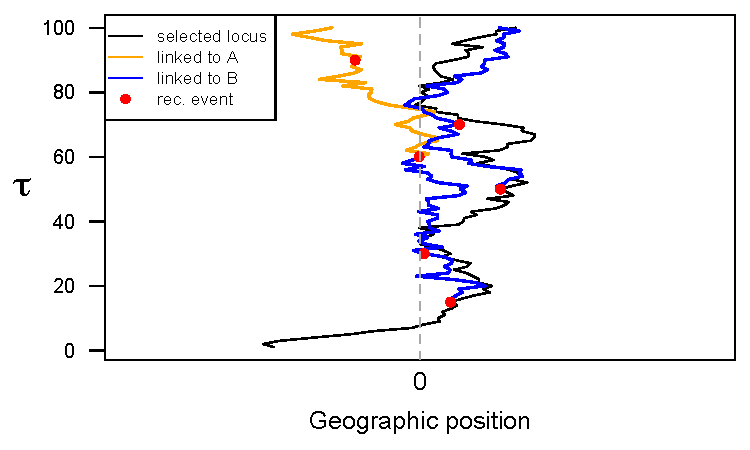
\includegraphics{figs/BM_schematic}
\caption{A cartoon representation of a haplotype under the model. The black line represents the path, backwards in time, of a site under selection ($L_B$) that is sampled in the present day ($\tau=0$). The center of the hybrid zone is defined at geographic position $x=0$, such that ancestry A segregates at lower frequency for $x>0$. Here, because of negative selection, $L_B$ migrates rapidly back to $x>0$ from a position $x<0$. Red dots represent recombination events along the entire haplotype, and lineages that recombine off the same haplotype as $L_B$ are represented by colored lines. (here, the initial haplotype is broken up into 3 chunks over 100 generations). Subsequent recombination events can cause these chunks to change which allele they are linked to at the selected site, and here yellow lineages are linked to an allele of ancestry $A$ at the selected locus, and blue lineages are linked to a selected allele of ancestry $B$. From right to left, the chunks at $\tau=100$ are of ancestry $(A, B, B)$. }\label{Fig:schematic}
\end{figure}
%As an approximation, we consider a cline of narrow width (look up cline width for underdominance, Barton/May?), such that the frequency of migrant alleles is exponential and negligible at distance away from the center of the hybrid zone. This means that recombination events that occur away from the center of the zone do not result in a change in $a$.


%%%%%%%% %%%%%%%%%%
\subsection*{Analysis}

\plr{The aim here is to give both the heuristics, for how a lineage moves around
and what that tells us about the scale on which clines happen;
as well as writing down the PDE.  These should probably be better separated?}

Perhaps start out with the main points:
the cline takes time $s$ to spread out,
and after time $\tau$ will have clines out to genetic distance of order $1/\tau$,
maybe more. \alisa{has this not already been stated by Nick somewhere?}

\paragraph{Establishment of  \sout{the selected cline} \alisa{a cline at the selected locus}}
Consider a single locus, with alternate alleles fixed in the two parental populations,
for which heterozygotes have fitness $1-s$, and homozygotes are of equal fitness.
The deterministic theory predicts that after secondary contact,
these alleles will form a stable cline.
To study gene flow past this cline we first need to understand how the cline itself is formed.
Let $p(x,t)$ denote the frequency of the $A$ allele at spatial location $x$ and time $t$.  
Suppose that secondary contact occurred at time $t=0$, \alisa{(Will switching between backwards and forwards in time not get confusing?)}
and that $p(x,0) = 1$ if $x<0$ and $p(x,0)=0$ if $x>0$.
(In discrete computations, a deme at $x=0$ has $p(0,0)=1/2$.)
Let $\sigma^2$ be the mean squared distance between parent and offspring.
Assuming local random assortment of alleles into diploids,
that the habitat and dispersal are homogeneous,
and that $s$ and $\sigma$ are small, 
the commonly-used equation that $p$ solves is
\begin{align} \label{eqn:cline_pde}
    \dot p = \frac{\sigma^2}{2} \Delta p + s p (1-p) (2p-1) ,
\end{align}
where $\dot p(t,x)$ is the time derivative and $\Delta p$ is the Laplacian,
as derived in \citep{bazykin}; for discussion of diploidy see \citep{diploidcline}.
There is not an exact analytic solution to this equation, 
but a good approximation to the equilibrium solution is that
$\lim_{t \to \infty} p(x,t) \approx (1+\tanh(-2x\sqrt{s}/\sigma))/2$ \citep{bazykin}.
Considering the numerous approximations going into this,
the important attributes are that 
the stable cline has width of order $\sigma/\sqrt{s}$,
and decays exponentially.
Furthermore, the cline is established through diffusion \alisa{of individuals?}, which is slowed down somewhat by selection against heterozygotes,
but is still diffusive, and so it will take time of order $1/s$
to reach its stable width \alisa{(is this something that has been shown before?)} This can be shown by rescaling space by $\sigma/s$ and time by $1/s$ in equation \eqref{eqn:cline_pde}, and seeing that the result \alisa{(what result?)} doesn't depend on $\sigma$ or on $s$.

\paragraph{Lineages at the selected locus}
Now suppose that the frequency profile of the selected allele $p(x,t)$ is given.
We will understand how lineages of sampled individuals behave,
both at and away from the selected site,
by following lineages as they move between backgrounds,
as done for instance in \citet{selectioncoal,ralph2015patchy}.
Consider the collection of $A$ alleles found at location $x$.
The expected number of such alleles produced by location $y$ is proportional to 
the number of $A$ alleles at $y$ multiplied by the probability of dispersing from $y$ to $x$;
looking in the other direction, this is also the probability that an $A$ allele at $x$ had a parent at $y$.
In other words, lineages move as the random walk determined by dispersal,
but biased towards areas that produce more of the selected allele that they carry.
Making the same assumptions underlying equation \eqref{eqn:cline_pde},
we show in Appendix \ref{apx:lineage_derivation}
that the lineage of an $A$ allele moves as Brownian motion with speed $\sigma$
with drift $s \grad \log p(x,t)$ (i.e., it is pushed uphill on $\log p$ at speed $s$).
Since $p=1$ far from the zone to the left, 
and is proportional to $\exp(-x\sqrt{s}/\sigma)$ to the right,
then roughly, lineages on ``their own'' side wander randomly,
while lineages on ``the wrong'' side are pushed at constant speed $\sigma/\sqrt{s}$ 
back towards the side where they are more common.
Since an $A$ allele must by definition have been inherited from the $A$ side of the barrier 
at the time of secondary contact,
this push must get more intense the closer it is to the time of secondary contact.
Lineages of $B$ alleles do the same thing, of course, but in the opposite direction.

\paragraph{Lineages at linked loci}
The behavior of a lineage at a linked locus is similar,
except that when in heterozygotes the lineage may move between backgrounds:
if we follow back through time the lineage of a locus we find linked to an $A$ allele, 
it will first tend to be inherited from ancestors to the left (as $A$ lineages drift to the left),
but if it spends time in the clinal region where recombination may happen,
it may be found to have been inherited from a $B$-carrying individual,
whose ancestors will tend to be more from the right.
Suppose we sample an allele today at a locus at recombination distance $r$ to the selected site.
If $X_t$ is the location of its ancestor $t$ generations ago,
and $Z_t$ is the identity of the selected allele that ancestor carried,
then we say that $X$ moves as a diffusion pushed by either $\log(p)$ or $\log(1-p)$,
and that $Z$ jumps between $A$ and $B$ at rate either $r p$ or $r(1-p)$,
depending on the identity of $Z$.
In symbols,
\begin{align}
    \begin{aligned} \label{eqn:lineage_motion}
        dX_t &= \begin{cases}
             s \grad \log(p(X_t,t)) dt + dB_t \qquad & \text{if } Z_t = A \\
             s \grad \log(1-p(X_t,t)) dt + dB_t \qquad & \text{if } Z_t = B 
        \end{cases} \\
        \P\{ Z_{t+\epsilon} = B \given Z_t = A \} &= \epsilon r (1-p(X_t,t)) + O(\epsilon^2) \\
        \P\{ Z_{t+\epsilon} = A \given Z_t = B \} &= \epsilon r p(X_t,t) + O(\epsilon^2)  .
    \end{aligned}
\end{align}

\textbf{figure of a lineage moving back and forth?}

\paragraph{How fast do linked clines relax?}
Although loci not under selection can in principle spread across the cline unimpeded,
in practice it can take quite some time for even unlinked neutral loci to homogenize,
due to the decreased fitness of heterozygotes \citep{bartonbarrier}
and the relative slowness of diffusive movement \citep{Sedghifar2015}.
Suppose we sample across at cline $\tau$ units of time after secondary contact.
How far away from the selected locus do we expect to see clines that have begun to flatten out more
than the selected cline?
A linked cline will have begun to flatten out if there is an appreciable chance that
a lineage at the linked locus initially linked to an $A$ allele 
at some point has recombined from an individual carrying the $B$ allele.
This implies that loci closer than $1/\tau$ to the selected site
certainly won't have a substantially wider cline than the selected cline.
\plr{Figure showing this? 
    For instance, either: (a) time-genome heatmap of number of heterozygotes (from PDE);
    or (b) a few time-space heatmaps of frequencies at different values of r (from PDE);
    or (c) a few space-genome heatmaps of frequencies at different times (from sims)
}
Of course, this calculation assumes that every generation provides an opportunity for recombination 
onto the other background,
but only recombinations in heterozygotes will move the linked lineage between selected backgrounds.
Since heterozygotes for the selected allele are only found at high frequency in the cline,
and lineages are generally pushed away from the cline but have no bias far away,
the amount of time a lineage spends in heterozygotes should grow as $\sqrt{\tau}$ for large $\tau$,
and so the width of the genomic region showing clines about the selected locus could be 
substantially larger than $1/\tau$.
However, this distinction appears hard to observe for realistic parameter values.


\paragraph{PDE for linked clines}
Clines at linked sites are given by
the probability that 
an allele sampled $t$ generations after secondary contact at location $x$,
at recombination distance $r$ to a selected allele of type $z$
is inherited from an individual of ancestry $A$,
where $z$ can be either $A$ or $B$.
Denote this probability $q_z(x,t,r)$.
In other words,
\begin{align}
    q_z(x,t,r) = \P^x \{Z_t = A\} .
\end{align}
The description above implies that $q_r$ solves the equation
\begin{align}
    \begin{aligned}  \label{eqn:q_pde}
    \dot q_A(x,t,r) 
            &= \grad \log(p(x,t)) \cdot \grad q_A(x,t,r) 
                + \frac{\sigma^2}{2} \Delta q_A(x,t,r) 
            \\ &\qquad {} + 
                r (1-p(x,t))(q_B(x,t,r)-q_A(x,t,r))  \\
    \dot q_B(x,t,r) &= \grad \log(1-p(x,t)) \cdot \grad q_B(x,t,r) 
            + \frac{\sigma^2}{2} \Delta q_B(x,t,r)
            \\ &\qquad {} + 
            + r (1-p(x,t))(q_A(x,t,r)-q_B(x,t,r))  ,
    \end{aligned} \\
\end{align}
with boundary conditions $q_A(x,0,r)=1$ and $q_B(x,0,r)=0$.
We will have more use for the differential operators on the right-hand sides of these equations,
so write these also as 
$\dot q_A = G_r^A q_A + r (1-p) (q_A-q_B)$
and 
$\dot q_B = G_r^B q_B + r (1-p) (q_B-q_A)$.

\paragraph{Numerical computation}
To determine how the cline at a linked locus is expected to relax,
we can solve the partial differential equations \eqref{eqn:cline_pde} and \eqref{eqn:q_pde} numerically,
producing, for instance, a heatmap of expected local frequencies of $A$ ancestry
across space and time, as in Figure \ref{fig:pde_clines}.
Shown is the expected frequency of ancestry $A$ at location $x$ and time $t$ at a site at recombination distance $r$ from the selected site,
which we denote $p(x,t,r)$ and can compute as $p(x,t,r) = p(x,t) q_A(x,t,r) + (1-p(x,t)) q_B(x,t,r)$.

%%%%%%
\begin{figure}
    \begin{center}
       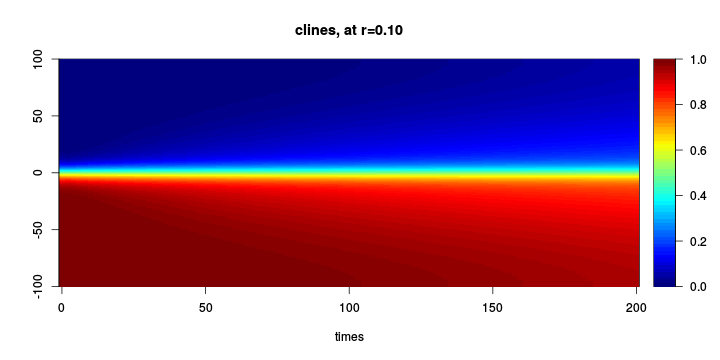
\includegraphics[width=0.7\textwidth]{figs/example_cline}
    \end{center}
    \caption{
        \textbf{Numerically computed clines,} at
        \textbf{(A)} the selected site, which forms over time $1/s$ and then remains stable, and
        \textbf{(B)} a linked site at distance $r=0.01$, which continues to smooth out as $\sqrt{t}$.
        \textbf{(C)} a linked site at $r=0.1$
        \textbf{(D)} an unlinked site.
        Other parameters.
       \plr{Do we want this figure? This one is just a placeholder; I'd put in two, that showed the formation and spread better.
       This is from the PDE (we don't have time courses from sims).}
        \label{fig:pde_clines}
    }
\end{figure}


\paragraph{Haplotype lengths}
We can also find the probability of seeing an entire block of genome (haplotype)
of a single ancestry at a given location and time.
As in \citet{Sedghifar2015},
to do this we need only keep track of both lineages when a recombination in the middle of a block occurs,
so that lineages will act like a particular class of labeled, branching diffusions,
where the total branching rate is conserved.
We will not consider subsequent coalescence.
The general description of the process is as follows.
The lineage of a segment of genome behaves as a linked locus described in equations \eqref{eqn:lineage_motion},
with recombination distance $r$ equal to the rate at which the segment recombines away from the selected site.
(If the selected site lies inside the segment, $r=0$.)
Additionally, at rate equal to the genetic length of the segment,
a recombination occurs, at which point the segment splits into two segments at a uniformly chosen location,
each of which procedes as before, independently.

\paragraph{Spatial haplotype patterns}
Furthermore, we expect that stretches of $A$ ancestry will tend to be shorter the further one moves into the $B$ side of the cline,
because they have had more opportunities to recombine with $B$ haplotypes.
However, stretches of $A$ ancestry that contain the selected site are expected to be longer
than those that do not at the same spatial location,
because lineages containing the selected site must have been inherited from the $A$ side of the cline recently --
concretely, they move at speed roughly $\sigma/\sqrt{s}$,
so we expect (selected) $A$ alleles at distance $x$ from the cline center
to have last had an ancestor on the $A$ side of the cline around $x \sqrt{s}/\sigma$ generations ago,
and so the enclosing $A$ haplotype is no longer than $\sigma/(x \sqrt{s})$.
\plr{(check predicted decay of mean length $1/x$ in simulations)}
For linked haplotypes not containing the selected site, the situation is more complicated, and harder to intuit.

\paragraph{General haplotype probabilities}
To quantify haplotype abundances,
we'd like to know the probability that the entire segment of genome between positions $a$ and $b$ relative to the selected site
in an individual sampled at spatial location $x$ and time $t$ after the cline has formed
is of ancestry $A$.
Writing this probability $g_A(x,t;a,b)$,
branching adds a term to equation \eqref{eqn:q_pde}, so that 
\plr{write this equation more compactly?}
\begin{align}
    \begin{aligned} \label{eqn:g_pde}
        \dot g_A(x,t;a,b) 
            &= G_{r(a,b)}^A g_A(x,t;a,b) 
            - (b-a) g_A(x,t;a,b) 
            \\ {} & \qquad 
            + p(x,t) \int_a^b {
                g_A(x,t;a,\theta) g_A(x,t;\theta,b) 
                - g_A(x,t;a,b) .
            } d\theta
            \\ {} & \qquad 
            + (1-p(x,t)) \int_a^0 {
                g_B(x,t;a,\theta) g_A(x,t;\theta,b)
            } d\theta
            \\ {} & \qquad 
            + (1-p(x,t)) \int_0^b {
                g_A(x,t;a,\theta) g_B(x,t;\theta,b)
            } d\theta,
    \end{aligned}
\end{align}
where the integral $\int_a^0$ is zero if $a>0$ and the integral $\int_0^b$ is zero if $b<0$;
and $r(a,b)$ is the distance from the segment to the selected site:
$r(a,b)=0$ if $ab<0$ and $r(a,b)=\min(|a|,|b|)$ otherwise.
The equation for $g_B(x,t;a,b)$ is identical after exchanging $A \leftrightarrow B$ and
$p \leftrightarrow (1-p)$.
The boundary conditions are $g_A(x,0;a,b)=1$ and $g_B(x,0;a,b)=0$.

\paragraph{Numerical solutions}
Notice that equations \eqref{eqn:g_pde}
are hierarchical in $[a,b]$:
the equation for haplotype identity probabilities on a segment $[a,b]$ depends only on those probabilities for smaller segments.
This allows for efficient numerical solutions,
described in more detail in Appendix \ref{apx:haplotype_calcs}.

%%%%%%
\begin{figure}
    \begin{center}
    \end{center}
    \caption{
        \textbf{Haplotype length distributions},
        comparing numerical solutions to simulations.
        At one time, plot 
        probability of seeing a haplotype of length at least $r$ covering that position on the genome,
        against (a) position on the genome, at a few spatial locations;
        or (b) spatial location, at a few positions on the genome.
        \plr{maybe?}
        \label{fig:haplotype_lengths}
    }
\end{figure}

\paragraph{Correlations in ancestry}
To compute correlations in local ancestry
(i.e., ``ancestry disequilibrium'', as in \citet{pool,brandvainthisvolume}),
we need only follow lineages at two sites, instead of an entire region,
the model described above requires only minor modifications,
and our numerical code can be used directly.


%%%%%%%% %%%%%%%%%%
\subsection*{Simulations}

We implemented forwards-time simulations of diploid individuals on a one-dimensional row of demes
with nonoverlapping generations and fixed population sizes (a Wright-Fisher model),
and a single locus with selection against heterozygotes in the center of one of two chromosomes, each of length 1 Morgan.
Each deme has exactly $n_d$ diploid individuals at the start of each generation.
Each generation,
first, each individual migrated to a new deme offset by $\lfloor Z + 1/2 \rfloor$ from their original position,
where $Z$ is a Gaussian random variable with mean zero and variance $\sigma^2$.
(The mean displacement is zero, and when comparing to theory we compute $\sigma$ as the standard deviation of this distribution.)
Migrants past either end of the range remained at the ends.
Then, 
fitnesses were computed (heterozygotes have fitness $1-s$; homozygotes have fitness 1),
and in each deme $n_d$ pairs of parents are chosen, with replacement,
with probability proportional to their fitness.
Selfing is allowed.
Since migration is not conservative, demes may have no available parents;
in this case, parents are chosen from other demes with probability proportional to fitness
multiplied by $\exp(-x^2/\sigma^2)$, where $x$ is the distance to the other deme.
The next generation is formed by carrying out meiosis in each parent
and combining the resulting gametes.
Meiosis results in alternating blocks of the gamete's chromsome
being inherited from the two parental chromosomes,
with the blocks separated by a Poisson(1) number of uniformly chosen recombination points along the chromosome,
and the order of the parental chromosomes chosen randomly.
The simulation software works by recording for each chromosome
a list of ancestry breakpoints and the index of the ancestor in the first generation
that the chromosome inherited that region of genome from;
genotyping at individual loci was performed by looking up the ancestor's genotype.

Hybrid zones of ages 10, 100 and 1000 generations were simulated under conditions of $\sigma=1$ and $s=0.1$. From this we measure unbroken tract lengths to the right of the selected locus. These were compared to the output of neutral simulations with $s=0$

\begin{figure}
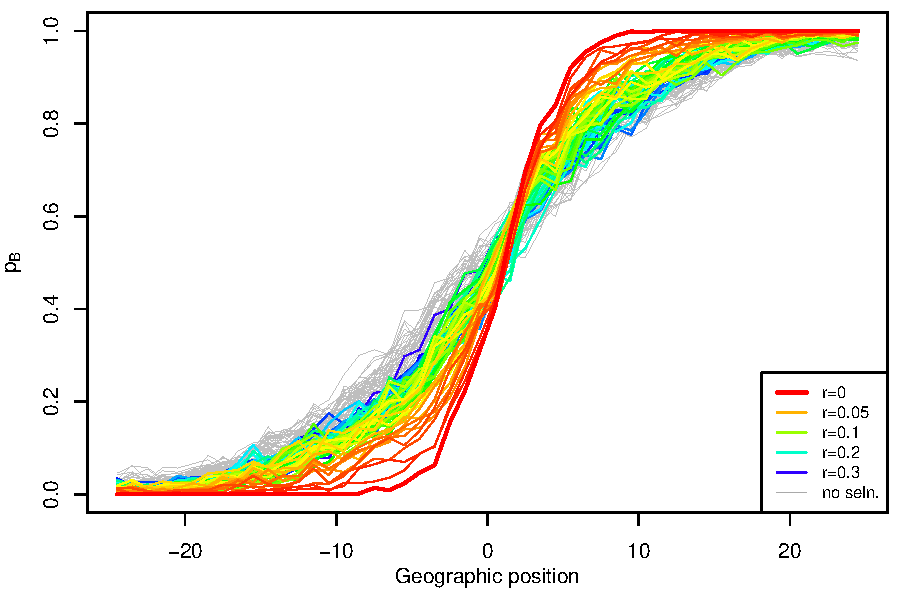
\includegraphics{figs/alleleFrequencies_sim}
\caption{Frequency of ancestry B at a given genomic and physical position at $\tau=100$. Every line represents a locus some distance $r$ away from the true target of selection, and $r=0$ represents the locus that is under selection. Grey lines represent the same positions from a similar simulation with no selection.}\label{alleleFreq_tau100}
\end{figure}

\subsection*{Statistics}
With the above theory and simulations, we are able to make predictions about patterns surrounding selected loci. In reality, however, such loci are not known, so it is useful to have per-site statistics that may allow for detection of candidate targets of selection. The most straightforward measure is $l_I(m)$ the length of haplotype chunk that a sampled chunk containing genomic position $b$, conditioned on ancestry $I$ at the site. Based on our expectation of the distribution of block lengths, we compute $l_B(m)$ for $m$ across a chromosome. 

Another statistic is the cumulative probability $C_I(m)$ of a sampled chunk encompassing position $m$ being longer than a chunk sampled from the distribution of all chunk lengths across the genome in the population. 

Additionally, we look at the mean value of these statistics in the two chunks, $m-$ and $m+$, that flank the block of unbroken ancestry containing $m$.



%\subsection*{Data}
%We compare the predictions of our model to genomic data obtained from individuals sampled a naturally occurring hybrid zone between \emph{Mus m. musculus/M. m. domesticus} \cite{Turner2011,Turner2014}. The genomic data generated by \citep{Turner2014} was for a mapping population generated by mating wild-caught individuals. Because some individuals were mated multiple times, the mapping population comprises many closely related individuals. We approximate wild population samples by restricting our analysis to genotyped individuals that had both parents sampled in the same location in such a way that none of the individuals shared a parent (see table for list of individuals). Approximately 280,000 SNPs were represented in the final dataset. 

%Ancestry blocks were estimated using ChromopainterV2 \cite{Lawson2012} and STRUCTUREv2 \cite{Falush2003} with $k=2$.


%Although we expect the age of this hybrid zone to correspond to historical human movement, and therefore be thousands of years old \cite{Teschke2008}, weighted the physical scale of ancestry-disequilibrium (both in the form of weighted ancestry-LD \citep{Loh2013} and ancestral block lengths) suggest relatively recent hybridization. Specifically, the high LD between quite distantly linked SNPs in the FS population suggests that a relatively high proportion of early-generation hybrids, whereas the rapid decay of LD in the the TU population reflects a much older hybridization event. Importance of geographic distribution of popgen patterns. 

%\begin{table}
%\begin{tabular}{l|c|c}
%Individual ID  & Population \citep{Turner2011} & Longitude(E)\\
%\citep{Turner2014}& \citep{Turner2011}&\\
%\hline
%FP112 & FS&11.665\\
%FP67 & FS &11.665\\
%FP114 & FS &11.665\\
%FP79 & FS &11.665\\
%FP152 &  FS &11.665\\
%FP11 & GL &11.965\\
%FP111&GL &11.965\\
%FP59 & HA  &11.721\\
%FP92 & HA &11.721\\
%FP7 &  HA  & 11.721\\
%FP45 & HA&11.721\\
%FP244& HO &11.693\\
%FP9&   RE&11.994\\
%FP5 &  RF&11.767\\
%FP78 &  SO &11.539\\
%FP52 &  SO &11.539\\
%FP180& SO &11.539\\
%FP14 & ST&11.539\\
%FP40 & ST&11.539\\
%FP145 & TU&11.748\\
%FP29&  TU&11.748\\
%FP135& TU&11.748\\
%\end{tabular}
%\end{table}

\section{Results}
\subsection*{The distribution of ancestry tract lengths}
We are interested specifically in the distribution of the length of continuous tracts of ancestry surrounding the selected locus. Far away from the zone center variants under negative selection will be rare \citep[for demonstration of this theoretical result, see e.g.][]{May1975,Slatkin1973,Barton??}, however, when present an unfit migrant haplotype is expected to be longer than a neutral migrant haplotype. Figure X shows the estimated probability density (pdf), of unbroken tract of ancestry B surrounding the selected locus, conditioning on a haplotype being of ancestry B at the selected locus. Compared to the expected density of tract lengths surrounding neutral loci, tracts of ancestry B around the selected locus are longer.

Of particular interest is whether or targets of selection could potentially be identified by a signal of larger ancestry tracts surrounding them compared to a genome-wide background. To demonstrate this, we simulated a chromosome of length 1M with a selected site at position 0.5M. For a set of positions $\mathbf{m}$ along the chromosome, we computed the length $l_B(m_i)$
of the surrounding unbroken block of ancestry. There is a detectable signal of increased block length surrounding selected loci when conditioning on the less-fit ancestry (Figure~\ref{Fig:blockLengths},~\ref{Supp:blockLengthHeatmap}) at geographic sites far from the center of the zone. A signal is also present for, but less well resolved when ancestry is not taken into account (Figures~\ref{Supp:blockLengthHeatmapNoAnc},~\ref{Supp:blockLengthNoAnc}).

\plr{or, perhaps for introduction?}
In addition to our finding that ancestry surrounding selected sites was quite long, our simulations revealed a consistent and unexpected finding. We found, on a given side of the hybrid zone, a transition from the locally adaptive ancestry at the selected site to the alternative ancestry at a closely linked site was short-lived (Figure~\ref{Supp:adjacentBlocks}). Put differently, blocks of `wrong' ancestry that do not overlap the selected site but are closely linked are exceptionally short. A simple intuitive explanation for this pattern suggests itself - loci physically linked to the selected sites can only survive on the wrong side of the hybrid zone for a reasonable amount of time if they recombine away from their ancestry at the locally adaptive site. Because it is then tightly linked to the alternate ancestry at the selected site, this ancestry chunk will large recombine with the alternate ancestry, and therefore decay rapidly. This pattern means that we can further refine the signal of block lengths around a selected locus, by measuring the ratio $\frac{2\sum{l_B(m_i)}}{\sum{l_A(m_i+)+l_A(m_i-)}}$ of mean block lengths surrounding a site with the mean length of adjacent blocks (Figures~\ref{Supp:ratioBlockAdjacent},~\ref{Supp:ratioBlockAdjacentHeatmap})




\begin{figure}
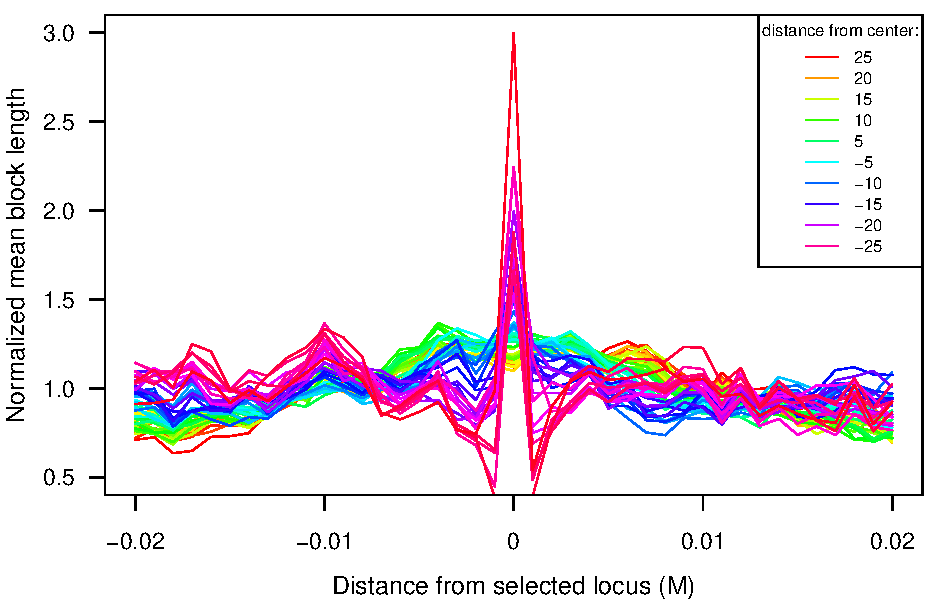
\includegraphics{figs/blocksAlongChromAncBConditioning}
\caption{Mean block length, $l_B(m_i)$, along a simulated chromosome of length $1M$ with selected locus at position $0.5M$. Here each line represents  $l_B(\mathbf{m})$, the mean block lengths in a given deme, and is normalized by mean block length $l_B(m_i)$ along the chromosome in the deme.}\label{Fig:blockLengths}
\end{figure}

\subsection*{Number of ancestors}
Although the theoretical model presented here does not account for coalescence, we are able to partially trace the genealogy of haplotypes in our simulations. In particular, we wish to know the relative number of ancestors from $\tau$ generations ago that are represented in present day populations at a given locus, given the frequency of a particular ancestry. This is a reflection of the average size of a haplotype family. We find that, as distance from the zone center increases, the average family size of an ancestor from time $\tau$ decreases (Figure~\ref{Fig:family_size}). One interpretation of this observation is that migrants tend to leave few offspring before being removed from the population by selection. 

\begin{figure}
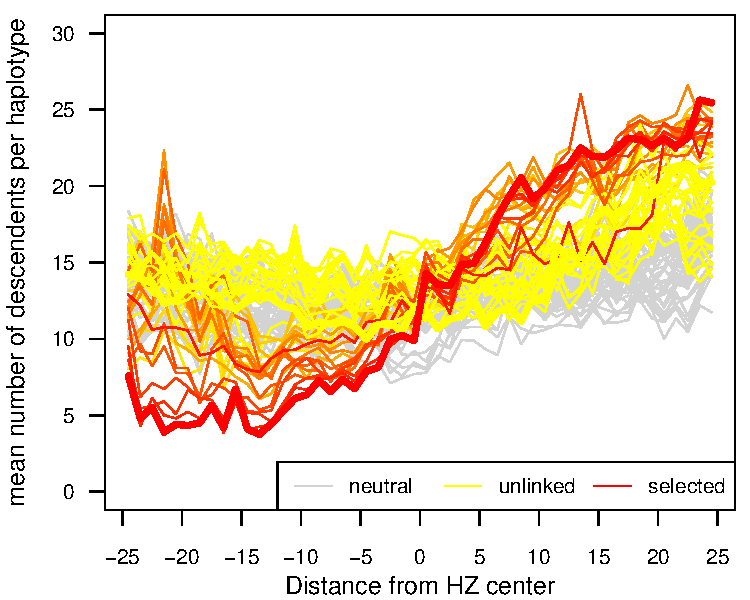
\includegraphics{figs/number_of_ancestors_tau1000}
\caption{The number of individuals of ancestry B per number of ancestors from $\tau=1000$ represented across geographic space. Each red or orange line represents a site some distance away (ranging from 0 - 0.01) from the selected site (here $s=0.01$ and $\sigma=1$). Yellow lines are corresponding positions on an unlinked chromosome with no selected loci, and grey lines are corresponding positions in a simulation with no selection.  Bold lines depict the target of selection when present, and corresponding position on chromosomes not harboring any selected sites.}\label{Fig:family_size}
\end{figure}

\subsection*{Identifying sites under selection}

Plots with x-axis the genome and having peaks at the selected site.

Question: how much resolution do we have?

\section{Discussion}
Here we present an expectation of ancestry block lengths in hybrid zones. We find that block lengths surrounding selected loci are, on average, longer than those surrounding neutral loci . This simply reflects the intuition that regions surrounding selected loci are going to have a harder time introgressing, and that further away from the center of the hybrid zone a haplotype containing a disadvantageous allele is likely to have been a relatively recent migrant and therefore will have experienced fewer recombination events.

Rapid drift (as in BM-drift) back to the `correct' side, conditional on being the wrong ancestry.

Something about how we just study the selection against hets model,
but we expect general conclusions to apply to other situations.

The tracking lineages given selection trick is an example of the more general idea of duality for particle systems.
It also assumes a large pop density limit that excludes recombination and makes lineages Markov;
if things are very patchy this might not be a good one.
Also, parent-offspring dispersal is not the same thing as successful-offspring-parent dispersal.


Topics include\\
- ignoring coalescent\\
- single locus model, selection is STRONG\\

Some words about how confidently calling tracts is the way of the future.\\
How can this be applied to detecting selection?

%% yaniv says:
\paragraph{Signals of block length}

\paragraph{Solutions to PDE}
Numerical solution for the PDE can be used on real, non-flat landscapes that change with time;
we have code and notes on solving them on github.

\bibliographystyle{molecularEcology}
\bibliography{library}

\appendix

\section{Rescaling a dicrete model to obtain the lineage motion}
\label{apx:lineage_derivation}

Here put derivation of the PDE for $p(x,t)$ and also the SDE of a lineage motion.

\section{Nuemrical solutions for haplotype probabilities}
\label{apx:haplotype_calcs}.

Here put some details about the numerical solutions of haplotype probabilities.

\end{document}
